%% Supplementary Exp-B iteration tables (appendix only).

Figure~\ref{fig:municipios-appendix} shows municipal hotspot counts for the Exp-B real-data subset. Tables~\ref{tab:exp-v1}--\ref{tab:exp-v7} document intermediate Exp-B iterations referenced in Section~\ref{sec:exp-b-synthetic}; Table~\ref{tab:three-class-full} gives the full sklearn report; Table~\ref{tab:ablation-neko} reports NeKo-PIGNN component ablation on synthetic Rothermel propagation data.

\begin{figure}[htbp]
\centering
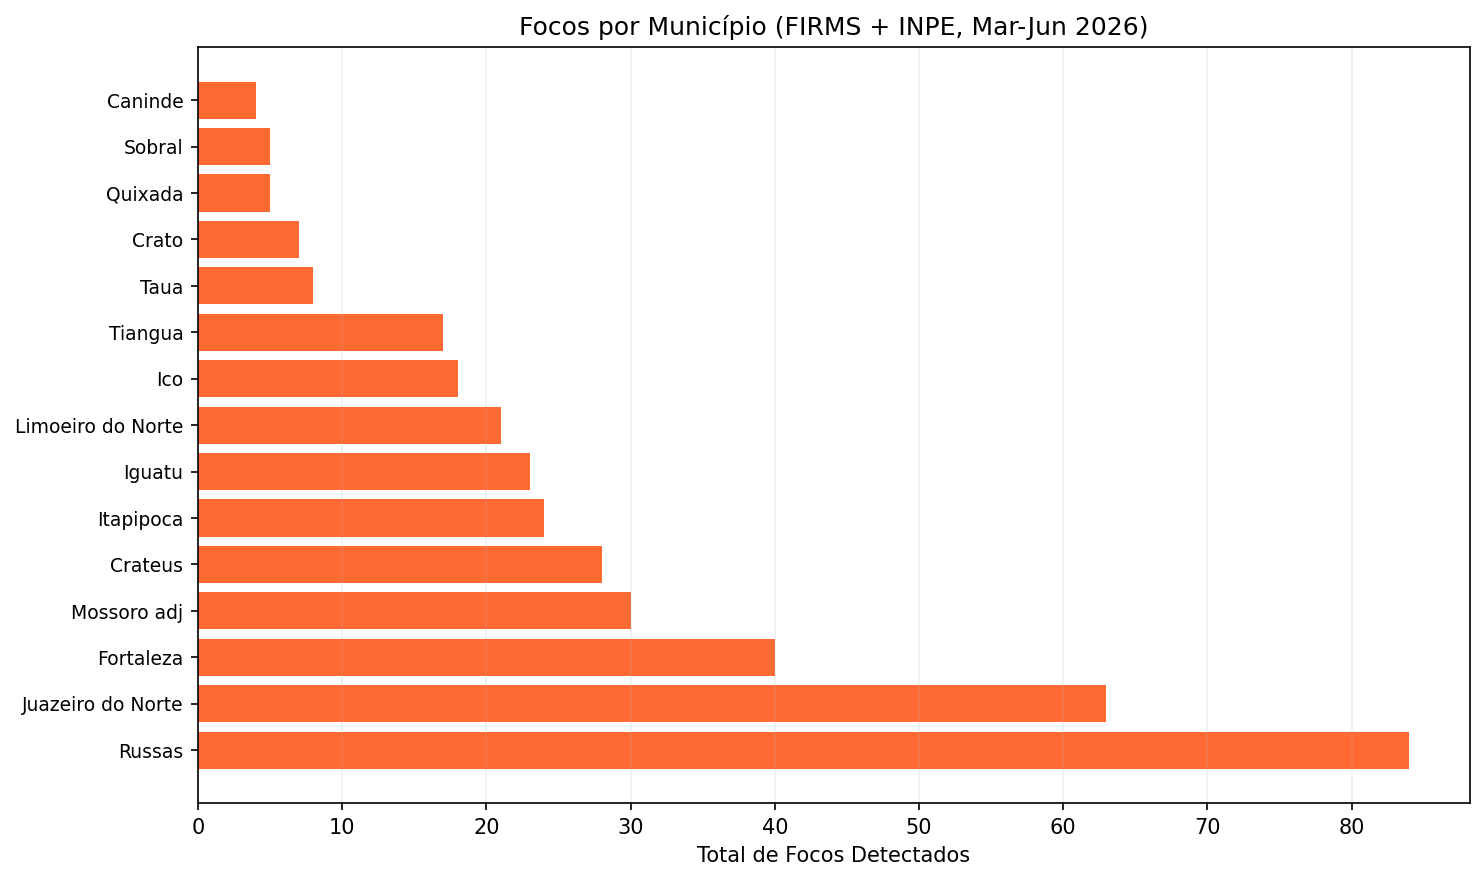
\includegraphics[width=0.75\linewidth]{figures/experimentos/05_focos_por_municipio.png}
\caption{Hotspots per monitored municipality (Exp-B real-data subset, Mar--Jun/2026).}
\label{fig:municipios-appendix}
\end{figure}

Table~\ref{tab:exp-v1} records the initial synthetic benchmark where KL-regularized Koopman-VAE underperformed shallow baselines. Table~\ref{tab:exp-v4} shows that feature expansion degraded MLP performance under data scarcity (62--67 training samples).

\begin{resulttable}{Exp-B v1: synthetic regression (200 steps, 20 nodes).}{tab:exp-v1}
\begin{tabular}{@{}lcccc@{}}
\toprule
\textbf{Model} & \textbf{RMSE}$\downarrow$ & \textbf{R\textsuperscript{2}}$\uparrow$ & \textbf{F1} & \textbf{Recall} \\
\midrule
MLP & \textbf{0.083} & \textbf{0.932} & 0.957 & 0.941 \\
XGBoost & 0.085 & 0.929 & \textbf{0.958} & 0.945 \\
Koopman-VAE (ours) & 0.260 & 0.343 & 0.828 & 0.989 \\
NeKo-PIGNN (ours) & 0.272 & 0.276 & 0.830 & 0.989 \\
\bottomrule
\end{tabular}
\end{resulttable}

\begin{resulttable}{Exp-B v4: real-data regression with feature-engineering variants.}{tab:exp-v4}
\begin{tabular}{@{}lcccc@{}}
\toprule
\textbf{Model} & \textbf{RMSE}$\downarrow$ & \textbf{R\textsuperscript{2}}$\uparrow$ & \textbf{F1} & \textbf{Precision} \\
\midrule
MLP plain & \textbf{0.143} & \textbf{0.782} & 0.936 & 0.911 \\
XGBoost + FeatEng & 0.149 & 0.767 & 0.935 & 0.902 \\
Ensemble (NeKo+XGB) & 0.149 & 0.766 & 0.930 & 0.896 \\
NeKo-PIGNN v3 & 0.173 & 0.686 & 0.906 & 0.907 \\
MLP + FeatEng + LB7 & 0.276 & 0.197 & 0.830 & 0.936 \\
\bottomrule
\end{tabular}
\end{resulttable}

Tables~\ref{tab:exp-v5}--\ref{tab:exp-v7} trace the rare-event detection iteration: v5 introduces Average Precision optimization; v6 adds focal loss and conservative XGBoost; v7 incorporates the persistence prior that raised precision to 47.5\% with only 21 false positives.

\begin{resulttable}{Exp-B v5: rare-event detection --- Average Precision and threshold metrics.}{tab:exp-v5}
\begin{tabular}{@{}lccccc@{}}
\toprule
\textbf{Model} & \textbf{AP}$\uparrow$ & \textbf{F1@best} & \textbf{Prec.} & \textbf{Recall} & \textbf{FP@0.3} \\
\midrule
MLP & 0.291 & 0.348 & 0.212 & 0.978 & 270 \\
NeKo-PIGNN v5 & \textbf{0.353} & 0.323 & \textbf{0.385} & 0.278 & \textbf{39} \\
XGBoost & 0.304 & 0.295 & 0.349 & 0.256 & 43 \\
Ensemble (NeKo+MLP) & \textbf{0.325} & \textbf{0.345} & 0.455 & 0.278 & --- \\
\bottomrule
\end{tabular}
\end{resulttable}

\begin{resulttable}{Exp-B v6: precision--recall operating modes.}{tab:exp-v6}
\begin{tabular}{@{}lccccc@{}}
\toprule
\textbf{Model} & \textbf{AP} & \textbf{F1@best} & \textbf{Prec.} & \textbf{Recall} & \textbf{FP@0.3} \\
\midrule
XGBoost (300 trees) & \textbf{0.322} & \textbf{0.427} & \textbf{0.335} & 0.589 & \textbf{28} \\
Ensemble (NeKo+XGB+MLP) & 0.315 & 0.353 & 0.217 & \textbf{0.956} & 67 \\
NeKo-PIGNN (5-seed avg.) & 0.280 & 0.324 & 0.233 & 0.533 & 81 \\
MLP (5-seed) & 0.276 & 0.350 & 0.213 & 0.989 & 282 \\
\bottomrule
\end{tabular}
\end{resulttable}

\begin{resulttable}{Exp-B v7: persistence prior combined with ML ensemble.}{tab:exp-v7}
\begin{tabular}{@{}lcccc@{}}
\toprule
\textbf{Model} & \textbf{Precision} & \textbf{Recall} & \textbf{F1} & \textbf{FP} \\
\midrule
Persistence only & 45.1\% & 48.7\% & 0.469 & 45 \\
Ensemble $\times$ Persistence & \textbf{47.5\%} & 21.1\% & 0.292 & \textbf{21} \\
NeKo $\times$ Persistence & 40.7\% & 24.4\% & 0.306 & 32 \\
XGBoost raw & 33.5\% & 58.9\% & 0.427 & 105 \\
\bottomrule
\end{tabular}
\end{resulttable}

Table~\ref{tab:three-class-full} reports per-class precision/recall/F1 from argmax classification; operational YES alerts use $P(\text{YES})\geq 0.30$ instead (Section~\ref{sec:three-level}). Table~\ref{tab:ablation-neko} confirms synergistic Koopman--PI-GNN coupling (full F1 = 0.914 vs.\ Koopman-only 0.820).

\begin{resulttable}{Full three-class classification report (Exp-B v9, XGBoost, 420 samples).}{tab:three-class-full}
\begin{tabular}{@{}lcccc@{}}
\toprule
\textbf{Class} & \textbf{Precision} & \textbf{Recall} & \textbf{F1} & \textbf{Support} \\
\midrule
NO & 0.693 & 0.973 & 0.810 & 186 \\
UNCERTAIN & 0.669 & 0.674 & 0.671 & 144 \\
YES & 0.500 & 0.078 & 0.135 & 90 \\
\midrule
Macro avg & 0.621 & 0.575 & 0.539 & 420 \\
Weighted avg & 0.644 & 0.679 & 0.618 & 420 \\
\bottomrule
\multicolumn{5}{@{}l@{}}{\textit{Note:} Operational YES alerts use $P(\text{YES})\geq 0.3$ (82.1\% precision), not argmax class.} \\
\end{tabular}
\end{resulttable}

\begin{resulttable}{NeKo-PIGNN component ablation on synthetic Rothermel propagation data.}{tab:ablation-neko}
\begin{tabular}{@{}lcccc@{}}
\toprule
\textbf{Model} & \textbf{F1} & \textbf{IoU} & \textbf{RMSE} & \textbf{R\textsuperscript{2}} \\
\midrule
NeKo-PIGNN (full) & 0.9140 & 0.8418 & 0.1083 & 0.8102 \\
Koopman-only & 0.8200 & 0.6949 & 0.1531 & 0.6215 \\
PI-GNN-only & 0.7900 & 0.6529 & 0.1682 & 0.5394 \\
Pure GNN & 0.3678 & 0.2255 & 0.2851 & $-0.32$ \\
CNN U-Net & 0.4599 & 0.2990 & 0.2514 & $-0.03$ \\
\bottomrule
\end{tabular}
\end{resulttable}
